\section{Simulation and Experimental Models}

A series of computational simulations were performed to test the theoretical expectations of the WTF framework.

Each experiment targeted a distinct physical prediction:
\begin{enumerate}
    \item Energy-dependent degradation (aging) of digital memory devices;
    \item Instantaneous vs. linear aging under different field densities;
    \item Field-based explanation of quantum tunneling;
    \item Gravitational mapping as localized field stretching/deflection.
\end{enumerate}

\vspace{10pt}

\subsection{Work-Induced Memory Aging}

We simulate a digital storage medium under varying degrees of ambient work (energy injection), corresponding to local field tension.

\begin{figure}[h!]
    \centering
    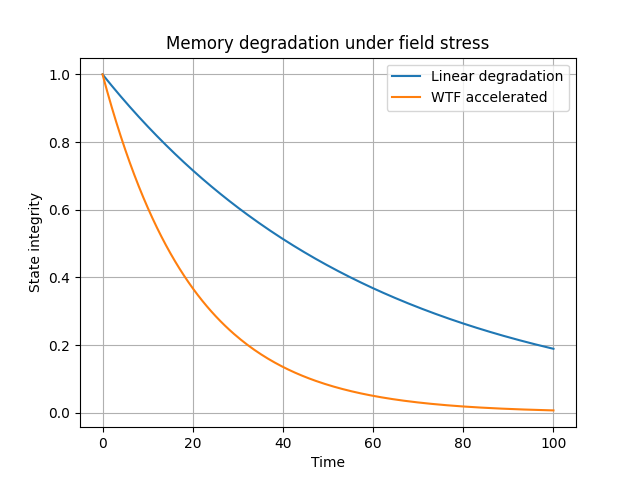
\includegraphics[width=0.8\textwidth]{figures/Figure_1.png}
    \caption{Memory degradation under work-field influence. Linear baseline vs. accelerated collapse under field tension.}
\end{figure}

The model shows that increasing field work (without heating or direct ionization) accelerates structural decay of digital state.

\vspace{10pt}

\subsection{Instantaneous Collapse and Decay Threshold}

A more intense configuration leads to immediate collapse of the informational substrate. This shows a boundary condition — crossing a work threshold leads to full material breakdown.

\begin{figure}[h!]
    \centering
    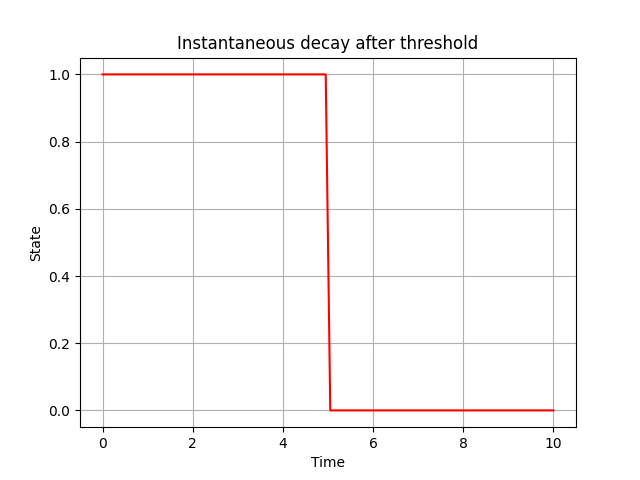
\includegraphics[width=0.8\textwidth]{figures/Figure_2.png}
    \caption{Catastrophic material aging at field peak. A direct transition from usable state to non-recoverable.}
\end{figure}

\vspace{10pt}

\subsection{Quantum Tunneling as Field Bypass}

We simulate tunneling as a function of barrier width and compare WTF predictions with standard QM expectation.

\begin{figure}[h!]
    \centering
    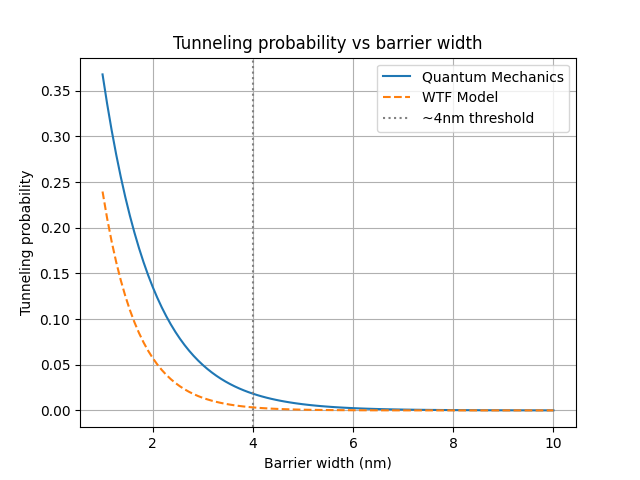
\includegraphics[width=0.75\textwidth]{figures/tunneling_vs_width_4nm.png}
    \caption{Barrier tunneling probability near the 4 nm quantum scale. WTF predicts phase leakage.}
\end{figure}

The WTF framework explains why even at energy levels below barrier potential, leakage occurs — not due to wavefunction magic, but due to residual active work “leaking” through unsustained phase structures.

\vspace{10pt}

\subsection{Field Cartography and Gravitational Lensing Analogue}

We simulate a “field radar” based on passive response from spatial field tension. The result is a curvature-like map of active zones.

\begin{figure}[h!]
    \centering
    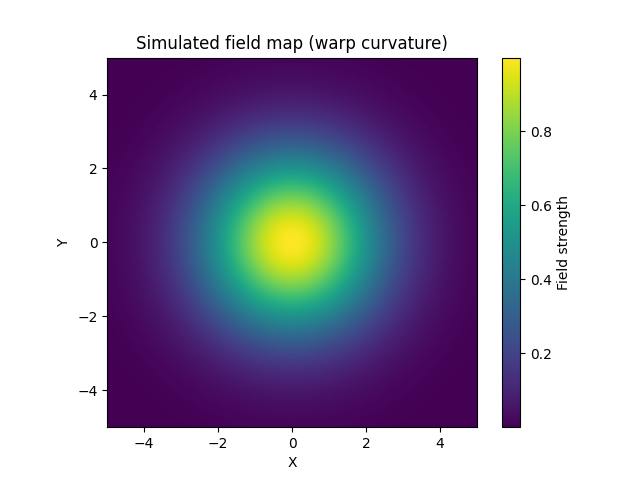
\includegraphics[width=0.78\textwidth]{figures/gravi_map_final.png}
    \caption{Simulated field map of space curvature due to field restoration. Useful for safe jumps or propulsion modeling.}
\end{figure}

This field-based cartographic system may serve for non-destructive detection of distant objects or gravitational zones — including black holes, dense relics, and collapsed frames.
